% Chapter 1

\chapter{Introducción general} % Main chapter title

\label{Chapter1} % For referencing the chapter elsewhere, use \ref{Chapter1} 
\label{IntroGeneral}

En este capítulo se presentan los conceptos fundamentales relacionados con los sistemas de alimentación automatizada para mascotas, el análisis del estado del arte, la motivación técnica y los objetivos que rigen el presente trabajo.

%----------------------------------------------------------------------------------------

% Define some commands to keep the formatting separated from the content 
\newcommand{\keyword}[1]{\textbf{#1}}
\newcommand{\tabhead}[1]{\textbf{#1}}
\newcommand{\code}[1]{\texttt{#1}}
\newcommand{\file}[1]{\texttt{\bfseries#1}}
\newcommand{\option}[1]{\texttt{\itshape#1}}
\newcommand{\grados}{$^{\circ}$}

%----------------------------------------------------------------------------------------

%\section{Introducción}

%----------------------------------------------------------------------------------------
\section{Introducción a los sistemas de alimentación automatizada}

El cuidado de mascotas en el hogar ha evolucionado significativamente gracias al avance de los sistemas embebidos y la electrónica de bajo costo. En particular, la alimentación de animales domésticos representa una de las principales preocupaciones de los propietarios, especialmente ante jornadas laborales extensas o ausencias prolongadas del hogar que dificultan el cumplimiento de rutinas nutricionales estrictas. La automatización de este proceso permite asegurar que los animales reciban la cantidad de alimento adecuada en los horarios correctos, independientemente de la presencia de sus dueños.

\subsection{Alimentación y bienestar animal}

Uno de los principales desafíos en el cuidado de gatos domésticos es garantizar una alimentación regular y controlada. Una rutina alimenticia inadecuada puede derivar en patologías frecuentes como la obesidad felina, la diabetes y los trastornos digestivos \cite{nutritional}, todas ellas asociadas a variaciones en la cantidad o los horarios de ingesta.

La medicina veterinaria establece que la ración diaria debe determinarse en función del peso, la edad y el estado de salud del animal, y distribuirse en momentos fijos del día para evitar ansiedad y alteraciones del comportamiento \cite{senior_pet_nutrition}. Conocer si el animal efectivamente consumió el alimento dispensado agrega una dimensión diagnóstica que los sistemas de alimentación tradicionales no contemplan.


\subsection{Domótica aplicada al cuidado de mascotas}

La domótica, entendida como la aplicación de tecnologías de automatización y control al entorno doméstico, ha experimentado un crecimiento sostenido en los últimos años \cite{smarthome}. La disponibilidad de microcontroladores de bajo costo, módulos de comunicación inalámbrica y sensores de alta precisión ha permitido extender estas soluciones a ámbitos que antes resultaban inaccesibles para el usuario común.

En el área específica del cuidado de mascotas, esta tendencia se traduce en dispositivos capaces de automatizar tareas rutinarias como la alimentación, la hidratación y el monitoreo de actividad, integrándose en muchos casos a plataformas de Internet de las Cosas (IoT) que permiten el acceso remoto desde dispositivos móviles.

%----------------------------------------------------------------------------------------

\section{Estado del arte}

En esta sección se presentan algunos productos disponibles en el mercado que abordan problemáticas similares a la planteada en este trabajo. Se realiza un análisis de sus características técnicas, limitaciones y diferencias respecto de la solución desarrollada.

\subsection{PetSafe Smart Feed}

PetSafe Smart Feed \cite{petsafe} es uno de los dispensadores automáticos para mascotas más difundidos en el mercado internacional. El dispositivo cuenta con conectividad Wi-Fi de 2,4 GHz y se gestiona mediante la aplicación móvil My PetSafe \cite{mypetsafe_app}, compatible con iOS y Android. Permite programar hasta doce raciones diarias con tamaños que van desde 1/8 de taza (29 ml) hasta 4 tazas (946 ml) por comida, y dispone de una capacidad de almacenamiento de 24 tazas (5 678 ml) de alimento seco o semihúmedo. La aplicación envía notificaciones ante nivel bajo de alimento, depósito vacío o pérdida de conectividad. La figura \ref{fig:petsafe} muestra el dispositivo, que se comercializa 
a un precio de USD~120{,}69.

\begin{figure}[H]
	\centering
	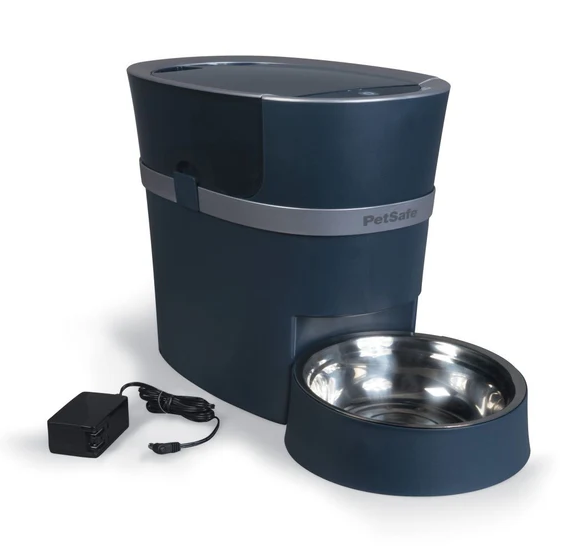
\includegraphics[width=10cm, height=10cm]{./Figures/PETSAFE.png}
	\caption{Dispensador automático PetSafe \textit{Smart Feed}.\protect\footnotemark}
	\label{fig:petsafe}
\end{figure}
\footnotetext{\url{https://www.petsafe.com/es/p/alimentador-de-mascotas-automatico-e-inteligente-smart-feed/PFD19-16861/}}

Sin embargo, el sistema no cuenta con ningún mecanismo de pesaje del plato, por lo que no es posible determinar si el animal consumió efectivamente el alimento entregado. El historial disponible en la aplicación refleja únicamente los eventos de dispensado, y el funcionamiento depende de manera permanente de una conexión a Internet.

\subsection{PETLIBRO Granary Wi-Fi}

El modelo PETLIBRO Granary \cite{petlibro} con conectividad Wi-Fi es un dispensador automático de alimento seco para gatos y mascotas de tamaño pequeño o mediano. Soporta redes de 2,4 GHz y 5 GHz, y permite configurar hasta diez comidas diarias con porciones ajustables de 20 ml, sobre una capacidad total de 5 litros. Su mecanismo de dispensado por paletas de distribución uniforme reduce la ocurrencia de atascos, y el sistema incorpora sellado cuádruple con bolsa desecante para preservar la frescura del alimento. Cuenta con batería de respaldo ante cortes de energía. La figura \ref{fig:petlibro} muestra el dispositivo, que se comercializa a un precio de USD~89{,}99 en el mercado estadounidense.

\begin{figure}[H]
	\centering
	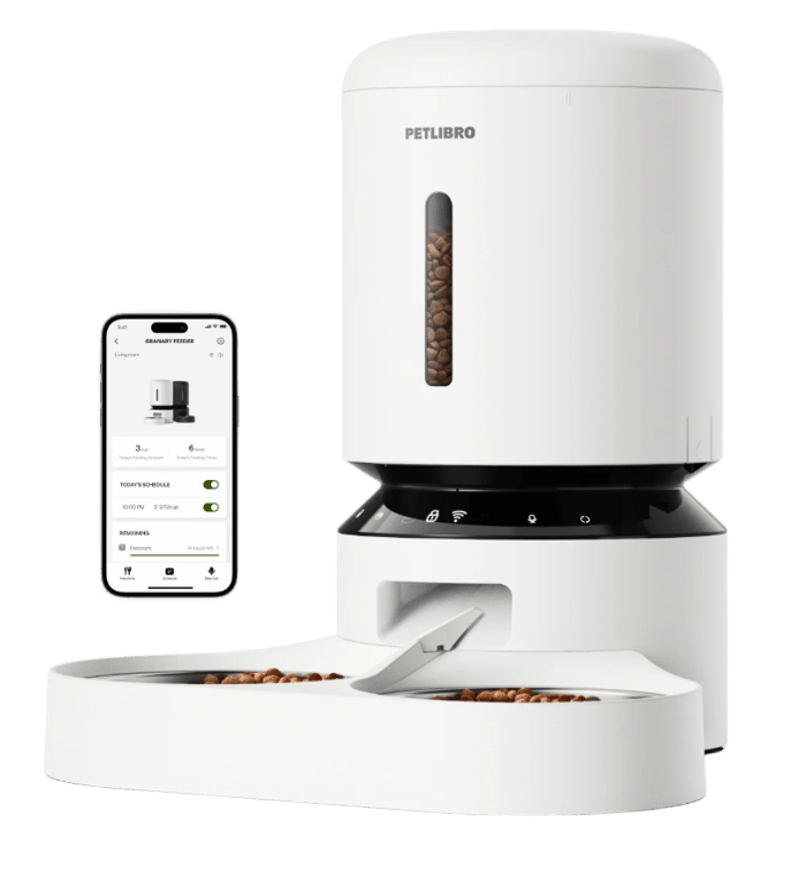
\includegraphics[width=9cm, height=9cm]{./Figures/PETLIBRO.png}
	\caption{Dispensador automático PETLIBRO \textit{Granary Smart Feeder}.\protect\footnotemark}
	\label{fig:petlibro}
\end{figure}
\footnotetext{\url{https://petlibro.com/products/petlibro-5g-wifi-automatic-pet-feeder}}

Al igual que el producto anterior, no incorpora un sistema de monitoreo del consumo real. El historial disponible en la aplicación registra únicamente los eventos de dispensado, sin ningún sensor que permita verificar si el animal ingirió efectivamente la ración entregada.

\subsection{Análisis del estado del arte y aportes del desarrollo}

Del análisis de los productos presentados se concluye que, si bien existen soluciones que automatizan la entrega de alimento con conectividad inalámbrica y control remoto, ninguna contempla la medición directa del consumo por parte del animal. Esta limitación impide obtener información confiable sobre el comportamiento alimenticio de la mascota, que es el dato de mayor valor para la detección temprana de alteraciones en su estado de salud. Adicionalmente, ambos productos analizados dependen de manera permanente de una conexión a Internet para operar, lo que los hace vulnerables ante cortes de conectividad o energía.

El sistema desarrollado en este trabajo incorpora como principal diferencial un módulo de pesaje del plato basado en una celda de carga HX711 \cite{hx711_datasheet}, que permite determinar con precisión si el alimento dispensado fue consumido. La gestión autónoma de horarios se logra mediante un reloj de tiempo real (RTC), lo que elimina la dependencia de Internet. La comunicación con el usuario se realiza a través de Bluetooth con una aplicación en PC, y la gestión eficiente de tareas concurrentes se implementa sobre FreeRTOS \cite{freertos_ref}. La tabla \ref{tab:comparacion_estado_arte}  presenta una comparación de las características principales entre los productos analizados y el sistema desarrollado.

\begin{table}[H]
\centering
\caption[Comparación de características entre productos del estado del arte y el sistema desarrollado]{Comparación de características entre productos del estado del arte y el sistema desarrollado.}
\footnotesize 
\begin{tabular}{l c c c}
\toprule
\textbf{Característica} & \textbf{PetSafe Smart Feed} & \textbf{PETLIBRO Granary} & \textbf{Sistema desarrollado} \\
\midrule
Conectividad             & Wi-Fi 2,4~GHz & Wi-Fi 2,4/5~GHz      & Bluetooth            \\
Raciones programables    & Hasta 12/día  & Hasta 10/día         & Por horario (RTC)    \\
Pesaje del plato         & No            & No                   & Sí                   \\
Dependencia de Internet  & Permanente    & Permanente           & No requerida         \\
Batería de respaldo      & No            & Sí                   & Sí                   \\
Dispensado manual        & No informado  & No informado         & Sí (pulsador físico) \\
Precio aproximado        & USD~120,69    & USD~89,99            & Bajo costo           \\
\bottomrule
\end{tabular}
\label{tab:comparacion_estado_arte}
\end{table}

Entre los aportes descritos, el módulo de pesaje del plato representa el diferencial más significativo, ya que ninguno de los productos comerciales analizados es capaz de determinar si el animal consumió efectivamente el alimento entregado. La operación autónoma ante cortes de conectividad y el bajo costo de implementación con componentes disponibles en el mercado local complementan esta ventaja, configurando una solución con potencial de aplicación tanto doméstica como clínica.
%----------------------------------------------------------------------------------------

\section{Motivación}

La motivación principal de este trabajo surge de la necesidad de contar con un sistema de alimentación para gatos que no solo automatice la entrega de comida, sino que también brinde información confiable sobre el comportamiento alimenticio de la mascota. Esta información resulta valiosa tanto para el propietario como para el veterinario, ya que permite detectar anomalías en el consumo que podrían indicar alteraciones en el estado de salud del animal.

Por otra parte, la disponibilidad de microcontroladores de alta capacidad, módulos de comunicación inalámbrica y sensores de precisión a precios accesibles representa una oportunidad para desarrollar soluciones tecnológicas que superen las limitaciones de los productos comerciales existentes. La Carrera de Especialización en Sistemas Embebidos de la FIUBA brindó las herramientas conceptuales y prácticas necesarias para llevar adelante un desarrollo de este tipo con rigor técnico y metodológico.

\section{Objetivos y alcances}

Este trabajo tuvo como objetivo desarrollar un prototipo funcional de un dispensador inteligente de alimento seco para gatos, basado en un microcontrolador STM32F446RE \cite{stm32f446re_datasheet}, que permita automatizar la entrega de comida en horarios programados, monitorear el consumo mediante el pesaje del plato y comunicar la información al usuario a través de Bluetooth.

El trabajo integró los conocimientos adquiridos en la Carrera de Especialización en Sistemas Embebidos de la FIUBA y abarcó el diseño del hardware, la implementación del firmware en lenguaje C sobre FreeRTOS y la validación del sistema mediante pruebas funcionales.

Por otra parte, no forma parte de este trabajo el desarrollo de una aplicación móvil completa ni de una plataforma web. Tampoco se contempla el diseño definitivo de la estructura mecánica del dispositivo, ni su adaptación para uso comercial.